\chapter{Implementazione proposta}
\label{chap:implementazione}
\vspace{1cm}
Il Capitolo \ref{chap:approccio} è stato interamente dedicato alla descrizione 
dell'approccio adottato nel lavoro oggetto di questa tesi, al fine di 
realizzare un baseline scheduler che tenga conto di possibili 
\emph{riconfigurazioni} e \emph{comunicazioni}, capace di fornire una 
valutazione quantitativa della bontà di un dato mapping.

Questo capitolo è dedicato alla descrizione dei dettagli implementativi 
riguardanti la realizzazione dell'algoritmo di scheduling.

Il capitolo è strutturato nel seguente modo: la Sezione 
\ref{sec:osservazioniGenerali} fornisce alcune osservazioni preliminari 
riguardo alle scelte implementative del progetto \ac{FASTER}; la Sezione 
\ref{sec:struttureDati} contiene la descrizione delle strutture dati relative 
all'implementazione dello scheduler; la Sezione \ref{sec:classiGerarchie} 
descrive le classi e le gerarchie che compongono la parte della toolchain 
relativa alla parte di mapping/scheduling (Sezione 
\ref{subsec:strutturaToolchain}) e i componenti dell'algoritmo di scheduling nel 
dettaglio (Sezione \ref{subsec:componentiScheduler}).


\section{Osservazioni generali}
\label{sec:osservazioniGenerali}
La maggior parte della toolchain di \ac{FASTER} è sviluppata in C++, 
linguaggio di programmazione a oggetti sviluppato da Bjarne Stroustrup 
\cite{CppStroustrup} come miglioramento del C, creato invece da Dennis Ritchie 
\cite{CKernighanRitchie}. La parte di interfaccia grafica, chiamata \emph{ASAP 
GUI} è sviluppata in C\#, linguaggio di programmazione ad oggetti sviluppato da 
Microsoft nell'ambito del \emph{framework .NET} \cite{ProCSharp}. ASAP GUI 
lancia degli script scritti in Python \cite{ThinkPython}, che si occupano di 
modificare l'XML del file di progetto come specificato dall'utente tramite 
l'interfaccia grafica.
% FIXME scrivere dei backend in python?
\paragraph{Convenzioni implementative della toolchain}
Riguardo allo sviluppo in C++ della toolchain di \ac{FASTER}, si è deciso di 
usare le strutture (\verb+struct+), per indicare tipi di dati dedicati alla 
memorizzazione di informazioni o utilizzati come ``contenitori''; le classi 
(\verb+class+) vengono utilizzate invece per rappresentare oggetti che hanno 
degli algoritmi al loro interno, invocabili come metodi.

\paragraph{Organizzazione dei namespace}
Nel codice si è deciso di includere le strutture e le classi dentro a 
\emph{namespace}, allo scopo di prevenire eventuali conflitti di nomi e di 
organizzare logicamente per categorie le varie parti della toolchain.

\begin{figure}
 \begin{center}
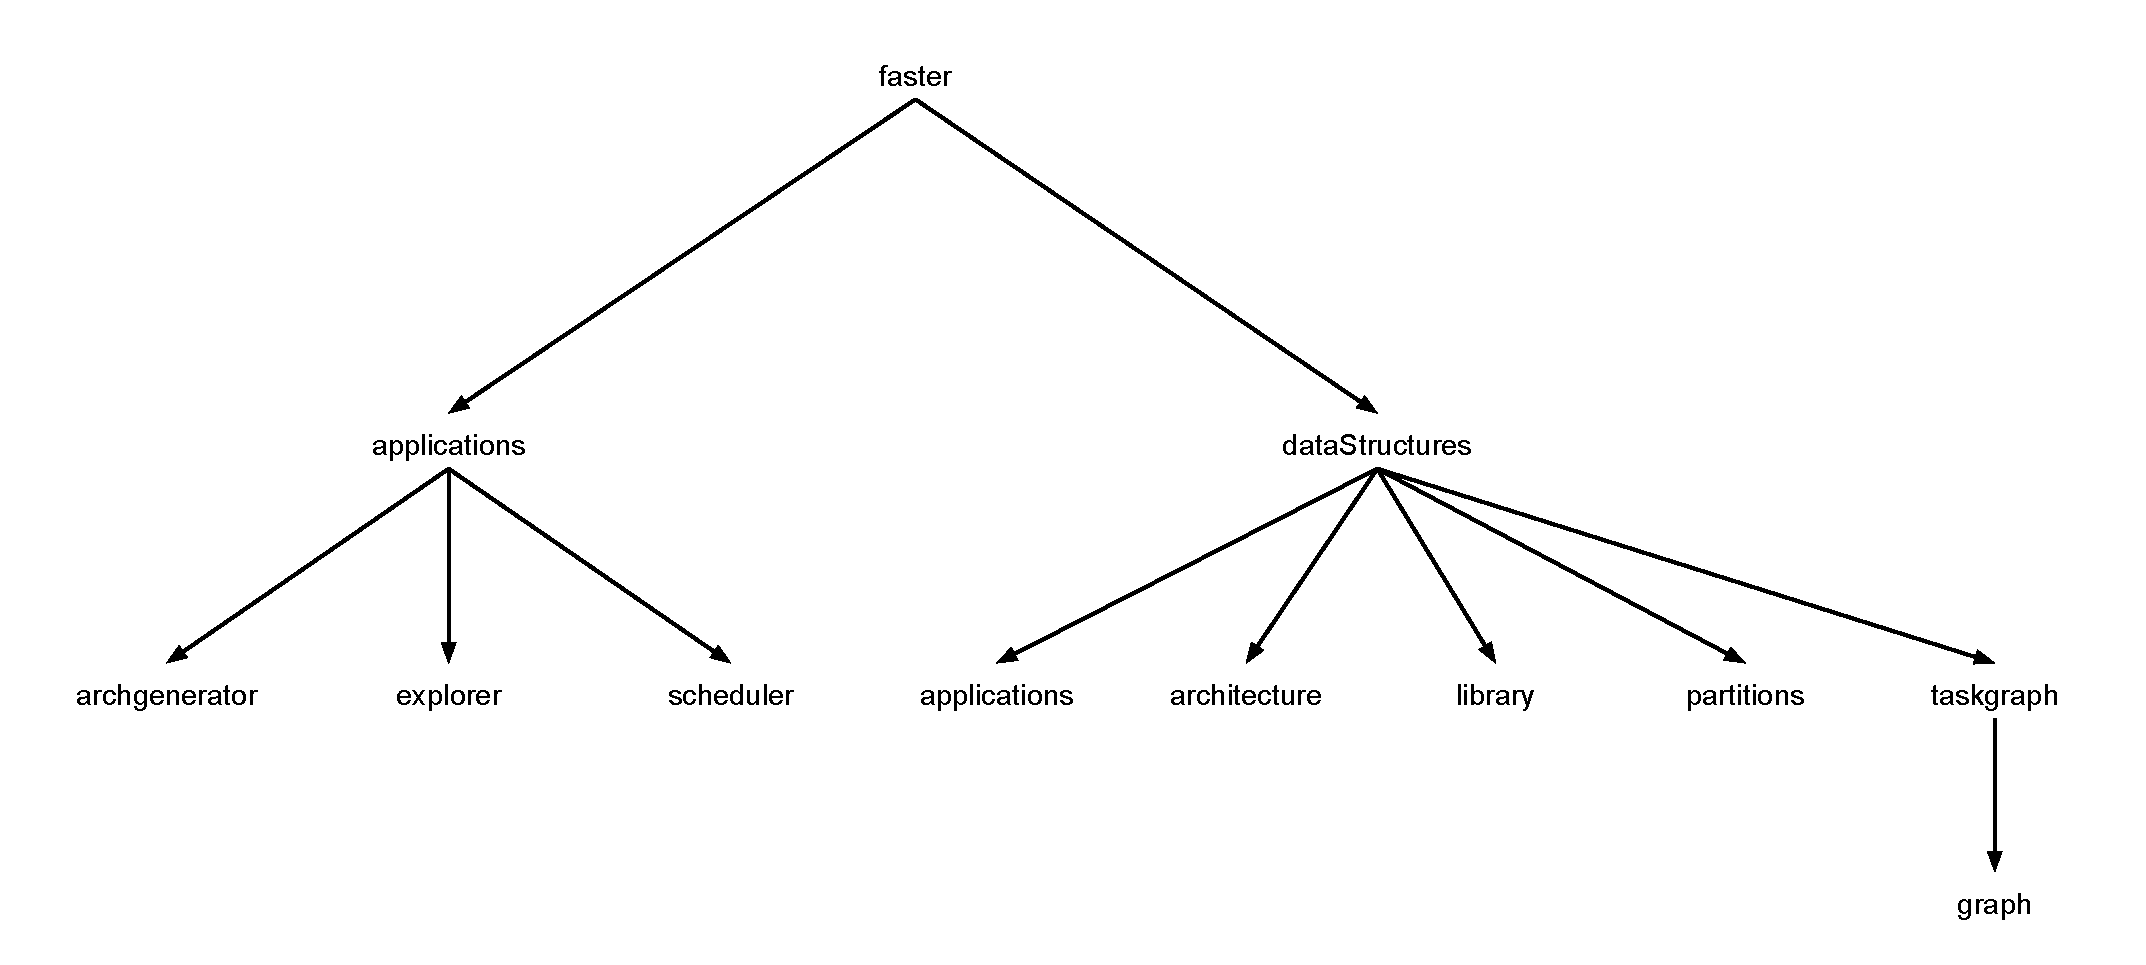
\includegraphics[width=\textwidth]{capitoli/figure/cap4/FASTERNamespaces.pdf}
\caption{Gerarchia dei namespace di \acs{FASTER}.}
\label{fig:gerarchiaNamespace}
 \end{center}
\end{figure}

Una rappresentazione della struttura dei namespace è visibile in Figura 
\ref{fig:gerarchiaNamespace}. La maggior parte di questi namespace verrà 
spiegata al momento di trattare classi o strutture che ne fanno parte 
e sono rilevanti per il lavoro oggetto della tesi.

% TODO parlare delle strutture dati di FASTER, prima o poi

\section{Strutture dati}
\label{sec:struttureDati}
L'obiettivo di questa sezione è presentare le più importanti strutture dati 
utilizzate dallo scheduler, che si trovano nella cartella 
\emph{toolchain/sources/common/datastructures/cpp/fasterInterfaces/scheduler}.

\subsection{Scheduler input}
I file \emph{schedulerInput.hpp} e \emph{schedulerInput.cpp} contengono la 
dichiarazione e l'implementazione della struttura \verb+SchedulerInput+, 
rispettivamente.


\section{Classi e gerarchie principali}
\label{sec:classiGerarchie}


\subsection{Struttura toolchain}
\label{subsec:strutturaToolchain}


\subsection{Componenti dello scheduler}
\label{subsec:componentiScheduler}

